\documentclass{beamer}
\usepackage{scrextend}
\usepackage{amsfonts}
%\usepackage[T1]{fontenc}
\usepackage{booktabs}
\usepackage[latin1]{inputenc}
\usepackage{graphicx}
\usepackage{mathtools}
\usepackage{multimedia}
\usepackage{url}
\usepackage{tikz}
\usepackage{pstricks,pst-node}
%Packages Tableaux
\usepackage{tabularx} %Tableaux
\usepackage{multirow} %Gestion des lignes
\usepackage{multicol} %Gestion des colones
\usepackage{fancybox} %Boites
\usepackage{multicol} %Colonnes
\usepackage{array} %Tableaux maths
\usepackage{fancybox}
\usetikzlibrary{arrows} 
\usetheme{Ilmenau}



\title[Monthly Meeting]{Inverse Procedural Generation of Geological Stories}
\author{Garcia Maxime}
%\institute{Mosig GVR}
%\date{January 2016}


\begin{document}

	
    \begin{frame}[label=(intro)]
	\titlepage
    \end{frame}
	
	
	\begin{frame}
	\frametitle{Today's agenda}
	\begin{itemize}
	\setbeamertemplate{itemize item}[ball]
	\item Current simulation results
	\setbeamertemplate{itemize item}[ball]
	\item Storytelling and geological events 
	\end{itemize}
	\end{frame}
	
	
	\section{Current results}
	
	\begin{frame}
	\frametitle{General pipeline}
    \begin{itemize}
    \item VPaint drawing analysis
    \item Story graph generation
    \item Simulation by choosing one path of the graph
    \item Success evaluation
    \item Animation export in VAC
    \end{itemize}
    \end{frame}
    
    
	\begin{frame}
	\frametitle{VPaint drawings examples}
	\begin{center}
	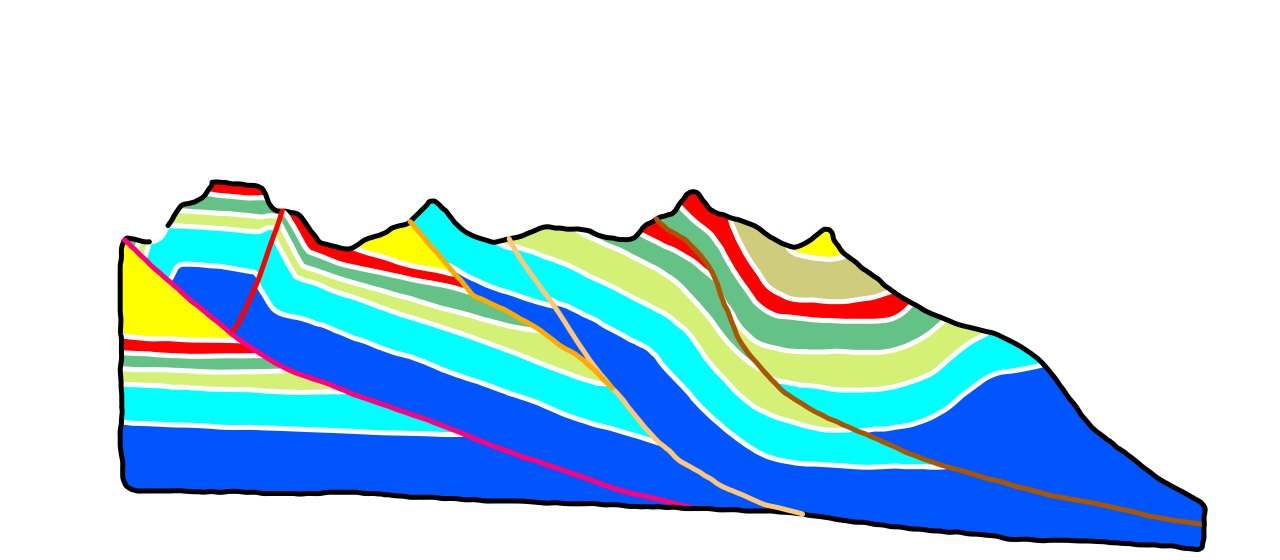
\includegraphics[scale=0.25]{chartreuse.png}\\
	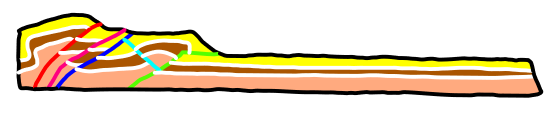
\includegraphics[scale=0.45]{bas1.png}
	\end{center}
	\end{frame}
	
	\begin{frame}
	\frametitle{Simulation Results}
	\url{miniChartreuse15.flv}
	\begin{itemize}
	\item Time step $dt = 0.0078$
	\item Torsion $(Tk) = 30$
	\item Stiffness $(k) = 10000$ for every materials 
	\item Friction $(f) = 0.2$ for every materials 
	\item External forces amplitude $= 5 $
	\item Merged layers are fixed 
	\end{itemize}
	\end{frame}
	
	\begin{frame}
	\frametitle{Simulation Results}
	\url{miniChartreuse5.flv}
	\begin{itemize}
	\item Time step $dt = 0.0078$
	\item Torsion $(Tk) = 30$
	\item Stiffness $(k) = 10000$ for every materials 
	\item Friction $(f) = 0.2$ for every materials 
	\item External forces amplitude $= 5$ 
	\item Merged layers are not fixed 
	\end{itemize}
	\end{frame}
	
    \begin{frame}
    \frametitle{VPaint drawing analysis}
    \begin{itemize}
    \item VPaint file input with color code
    \item Interlayers white colored
    \item Faults colored other than black or white
    \item Black egdes either ground surface or sketch boundaries
    %include chartreuse
    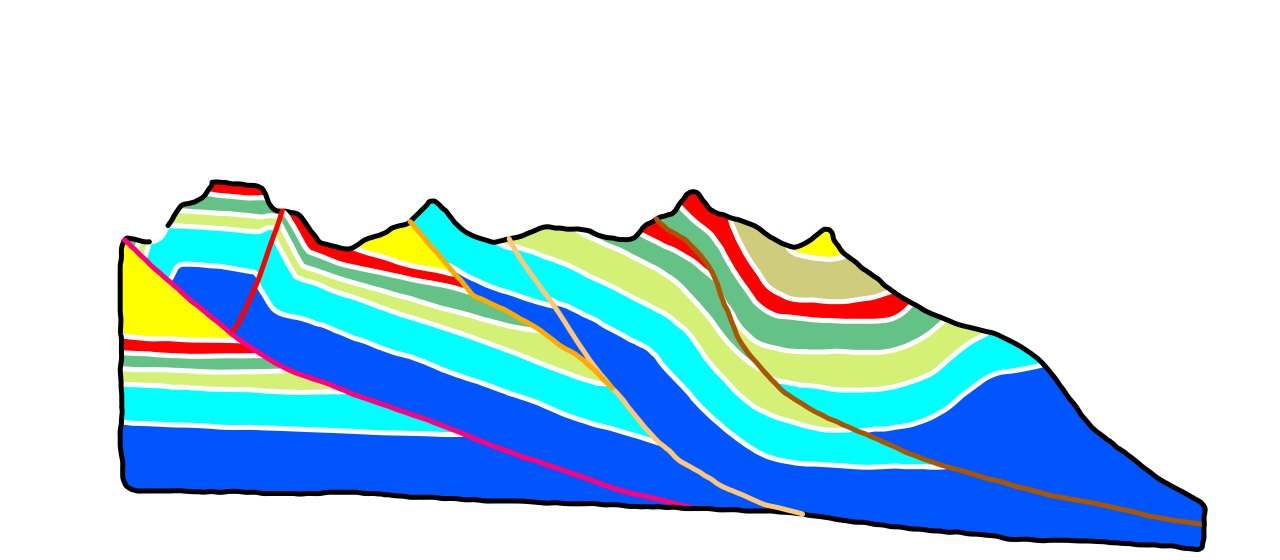
\includegraphics[scale=0.3]{chartreuse.png}
    \end{itemize}
    \end{frame}




	\begin{frame}
	\frametitle{Drawing topology extraction}
	\begin{itemize}
    \item Block structure detection: extract the block structure from the drawing
    \item Extract the different faults
    \item Identify upper and lower blocks in faults
    \item Complete extraction with information given by the user
    \end{itemize}
	\end{frame}	
	
	\begin{frame}
	\frametitle{Compaction Problem}
	\center{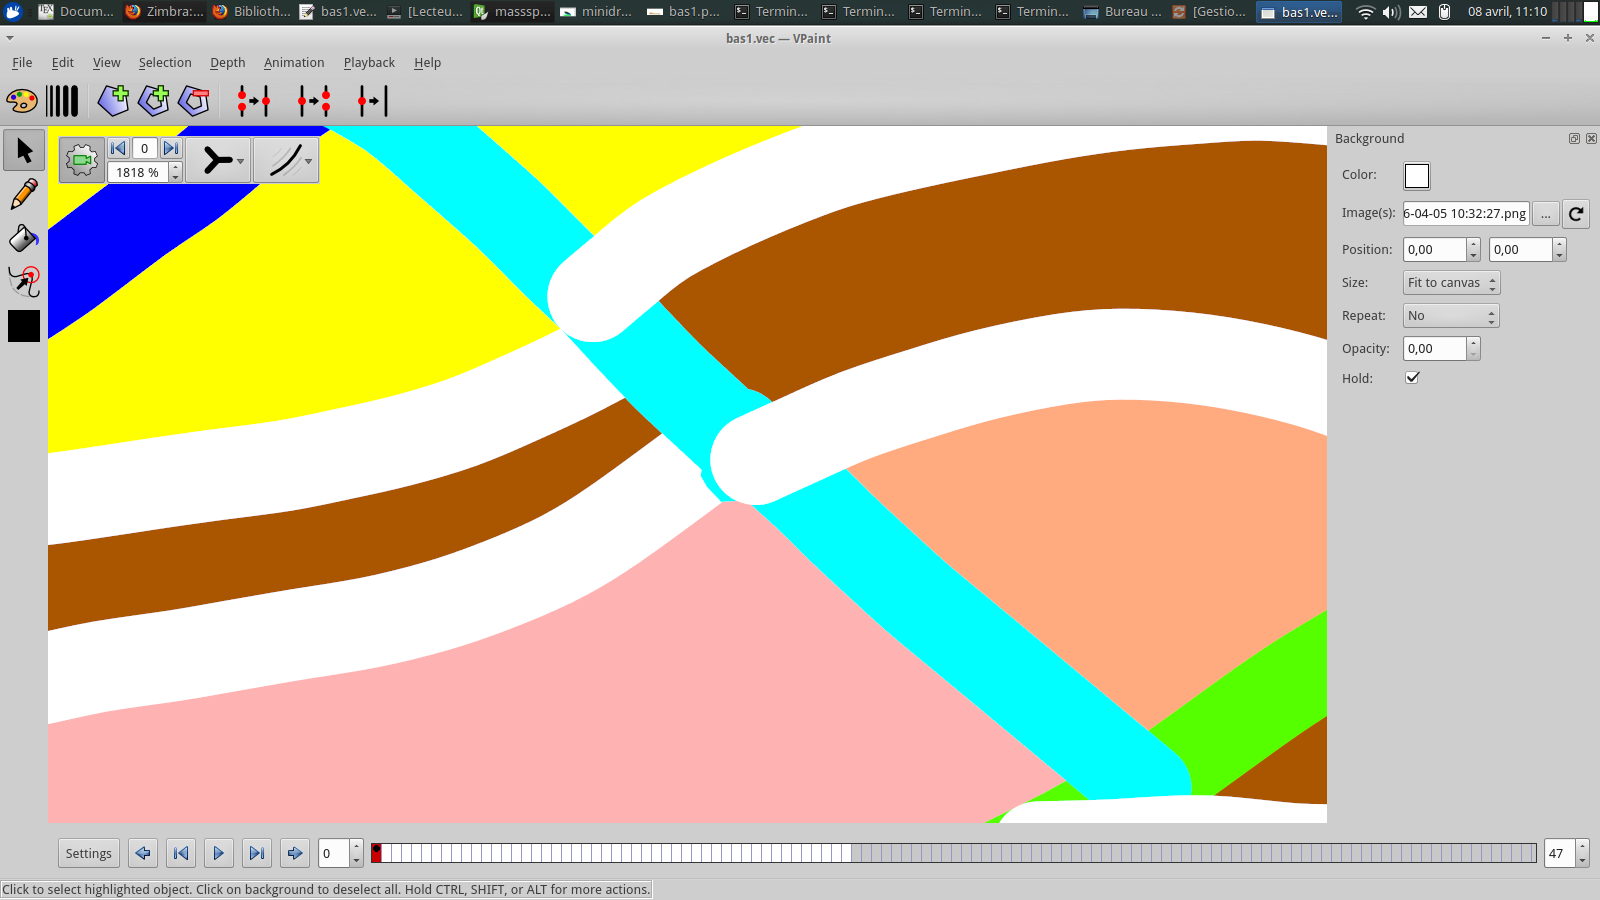
\includegraphics[scale=0.18]{compaction.png}}
	\end{frame}

	
	\begin{frame}
	\frametitle{Adding user information}
	\begin{itemize}
    \item Adding Material and Fault information
    %include screenshot material
     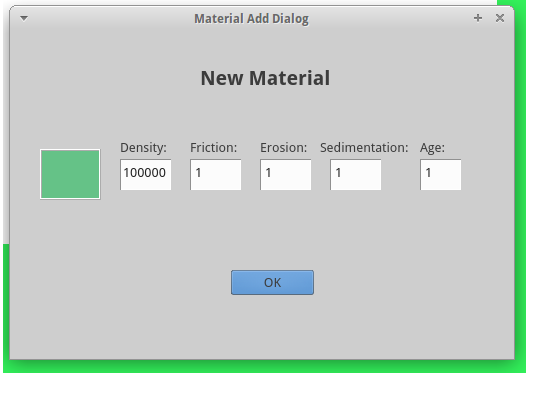
\includegraphics[scale=0.3]{materialDialog.png}
     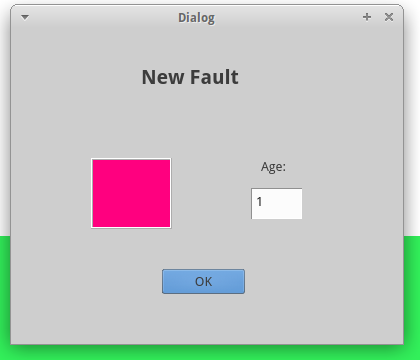
\includegraphics[scale=0.3]{faultDialog.png}
    \end{itemize}
	\end{frame}	
	
    \begin{frame}
	\frametitle{Simulation/Animation}
	\begin{itemize}
	\item Generate Mass-Spring system for each layer of each block 
	\item Run the simulation with several input parameters. Some come from the analysis (density, friction) and others are external but also configurable (dt, torsion, layer fusion condition, external forces)
	\item Simulate different kind of events (fault playing, pulling/pushing blocks, erosion/sedimentation, compaction)
	\end{itemize}
    \end{frame}

    
    \begin{frame} 
    \frametitle{Mass Spring generation exemple}
    \center{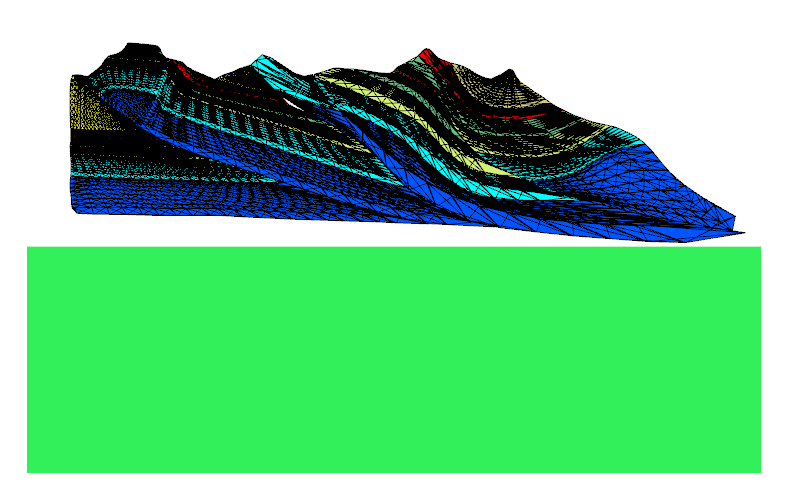
\includegraphics[scale=0.36]{chartreusespring.png}}
    \end{frame} 



	\section{Story Telling}	
	
	\begin{frame}
	\frametitle{Story Telling}
	\begin{itemize}
	\item Build a story graph of simulated events until no more event can be simulated (simulation end)
	\item Use user information to reduce the complexity (eg: Materials' ages)
	\item Use geological knowledge to reduce the complexity (eg: Fault hierarchy)
	\item At least 5 geological events to consider: Fault play, Compression/Expansion, Compaction, Sedimentation and Erosion.
	\item Consequently 5 events to simulate: UnFault ,UnCompress/ UnExpand, UnCompact, UnSediment and UnErode.
    \end{itemize}
	\end{frame}
	
	\begin{frame}
	\frametitle{Starting information}
	\center{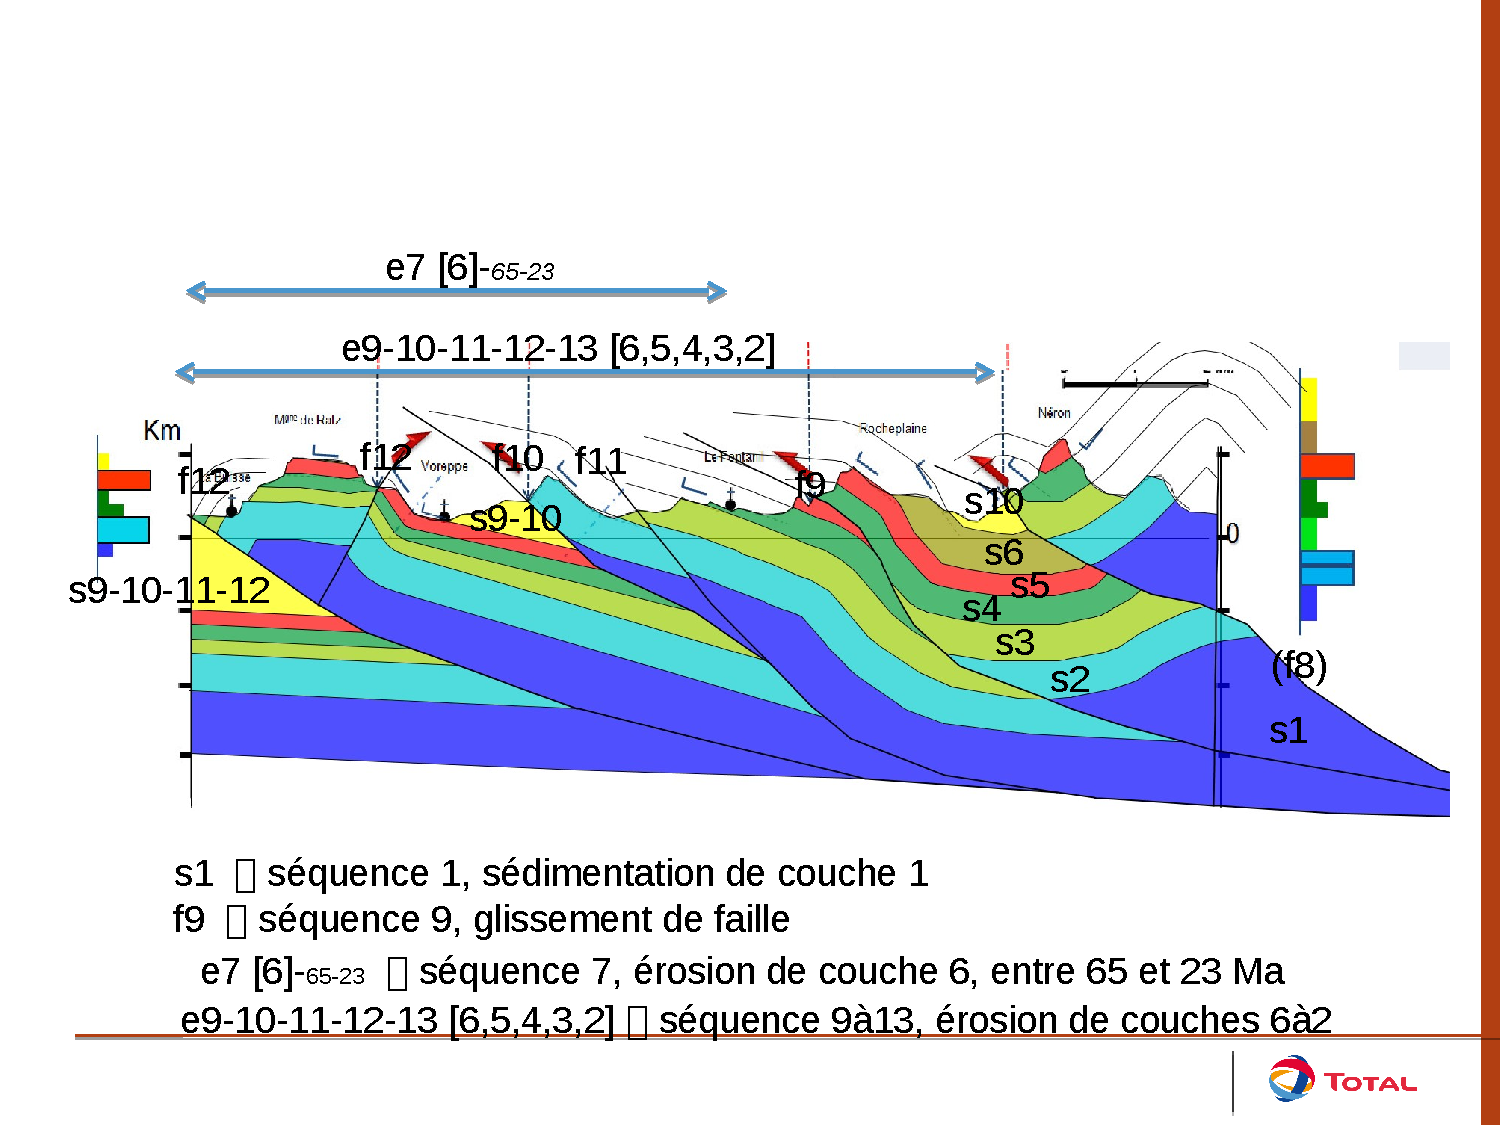
\includegraphics[scale=0.36]{Coupe_Chartreuse_rediscutee.pdf}}
	\end{frame}

	\begin{frame}
	\frametitle{Building the story}
	\begin{itemize}
	\item Two graphs to use in the story telling
	\item Event graph: show time dependencies between geological events. An event is represented by a node and an edge represents a dependency.
	\item Story graph: represents the event paths we can run the simulation on. a node represents the list of event we can simulate at time t and an edge represents the event simulated between two nodes. Event graph used in the creation of this graph.
	\end{itemize}
    \end{frame}	    
    
    \begin{frame} 
    \frametitle{Event Graph example}
    \includegraphics[scale=0.4]{eventGraph.pdf}
    \linebreak
    \linebreak
    \includegraphics[scale=0.4]{timeArrowRight.pdf}
    \end{frame}
    
    \begin{frame} 
    \frametitle{Story Graph example}
    \includegraphics[scale=0.4]{StoryGraph.pdf}
    \linebreak
    \linebreak
    \includegraphics[scale=0.4]{timeArrowLeft.pdf}
    \end{frame}
	
    \begin{frame}
    \frametitle{Using Graphs in the simulation}
    \begin{itemize}
    \item First provide the user a path of the story graph where the simulation succeed (that is to say until there are no possible event to trigger).
    \item The user can choose to expand the story graph by selecting other events at a precised node. 
    \item A given path can lead to failure if one chosen event cannot be simulated which implies that this path will not lead to a correct restoration.
    \end{itemize}
	\end{frame}
	
	\begin{frame}
	\frametitle{Questions}
	\begin{itemize}
	\item Can we determine a local order (hierarchy) for faults ? 
	\item How can we detect and apply erosion ? is erosion applied during the whole simulation ?
	\item Is sedimentation also applied during the whole simulation ?
	\item The simulation is parametrized and can have various results according to these parameters. Should we offer to the user to change the parameters as an event in the story graph ? 
	\end{itemize}
	\end{frame}
	
            
\end{document}